\subsection{POC 2: Auto-Complete Form Inputs for Conference Registration in Indico}

The second prototype aims at connecting Solid with the conference registration module in Indico. When registering for a conference an \gls{html} form is presented with fields previously defined by the conference manager, who deemed those fields necessary. A form always contains personal information of the name and email address, but is not limited to it and can even range to more sensitive information such as copies of personal identification documents. Information of this type has perfect motivation to remain in the hand of the owner and not be stored in a remote data store, uncontrollable and unknown to the registrants.

Therefore, the initial aim was to extend the registration module to allow storage of sensible information in a data pod, where the user has full control and can handle the data to their own liking. This was decided to not be viable and the prototype changed to allow the extraction of data from a data pod and then use this data to map it to input fields of an Indico conference registration form -- the functionality to then also store the data from the registration in the user's data pod and not in Indico was dropped. The reasons and comprehensive analysis will be shared after the architectural analysis, synthesis, and evaluation of the developed alternating \gls{poc} in the \textit{design} \ref{poc2:design} and \textit{analysis} \ref{poc2:analysis} sections of this chapter.

\subsubsection{Architectural Analysis and Synthesis}\mbox{}\\

TODO:
\vspace{0.5cm}
\paragraph{System Description}\mbox{}\\

The system pulls in a resource from a data pod in Turtle format, maps the received information to input fields in an \gls{html} form and fills in missing inputs or asks the user if the values should be replaced.

\vspace{0.5cm}
\paragraph{Features}\mbox{}\\

The core functionality of the module consists of the following features: 

\vspace{-3mm}
\begin{enumerate}
    \item A user can provide a the \gls{uri} to a public Turtle file
    \item A user can choose to accept or reject values pulled in when values already exist
\end{enumerate}
\vspace{-3mm}

These features allow the development of a module giving users the ability to pull in their WebID profile document and use the information provided in it to populate a conference registration.
\vspace{0.5cm}
\paragraph{Type of Users}\mbox{}\\

There is one type of user for this system, who is the user with a WebID profile and interested in using the existing information to fill in a form.
\vspace{0.5cm}
\paragraph{Context Diagram}\mbox{}\\

Other types of involved parties are the ones maintaining or developing the system and application. These are shown in the context diagram \ref{fig:poc-autocomplete-context_diagram}.

\begin{figure}[H]
    \centering
    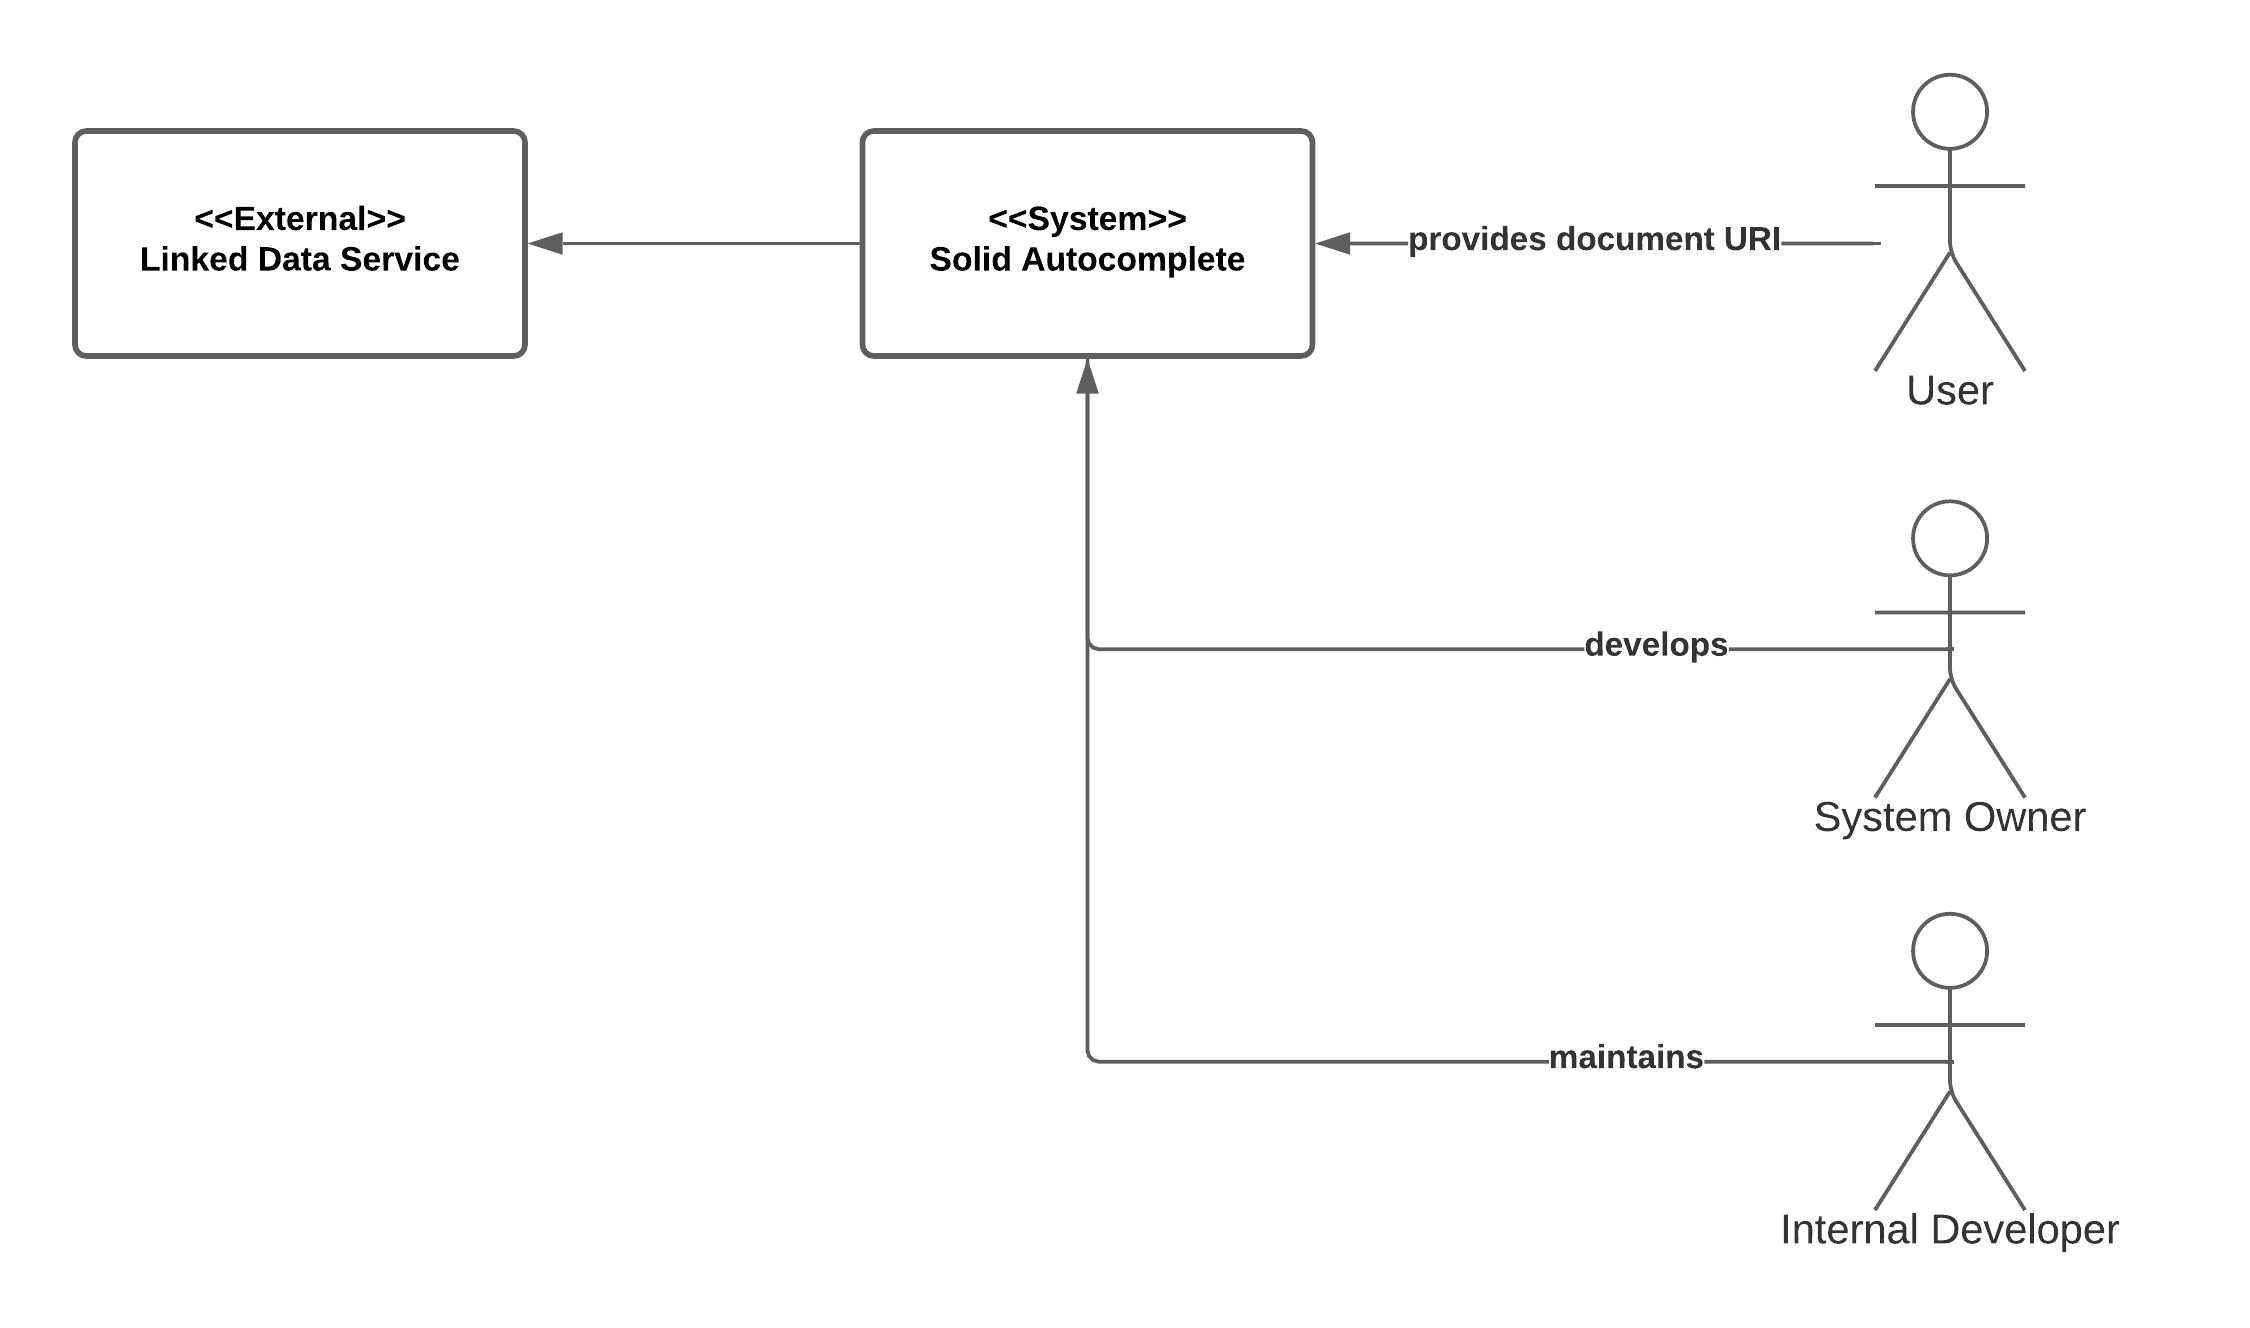
\includegraphics[width=0.8\textwidth]{prototype/graphs/poc-autocomplete-context_diagram.png}
    \caption{Context diagram showing users and external services of the system.}
    \label{fig:poc-autocomplete-context_diagram}
\end{figure}
\vspace{0.5cm}
\paragraph{Sequence Diagram}\mbox{}\\

The following succeeding diagram shows the sequential flow through the system upon initialization and button press. The focus was laid in the diagram to show the request/response cycles in the infrastructure. 

\begin{figure}[H]
    \centering
    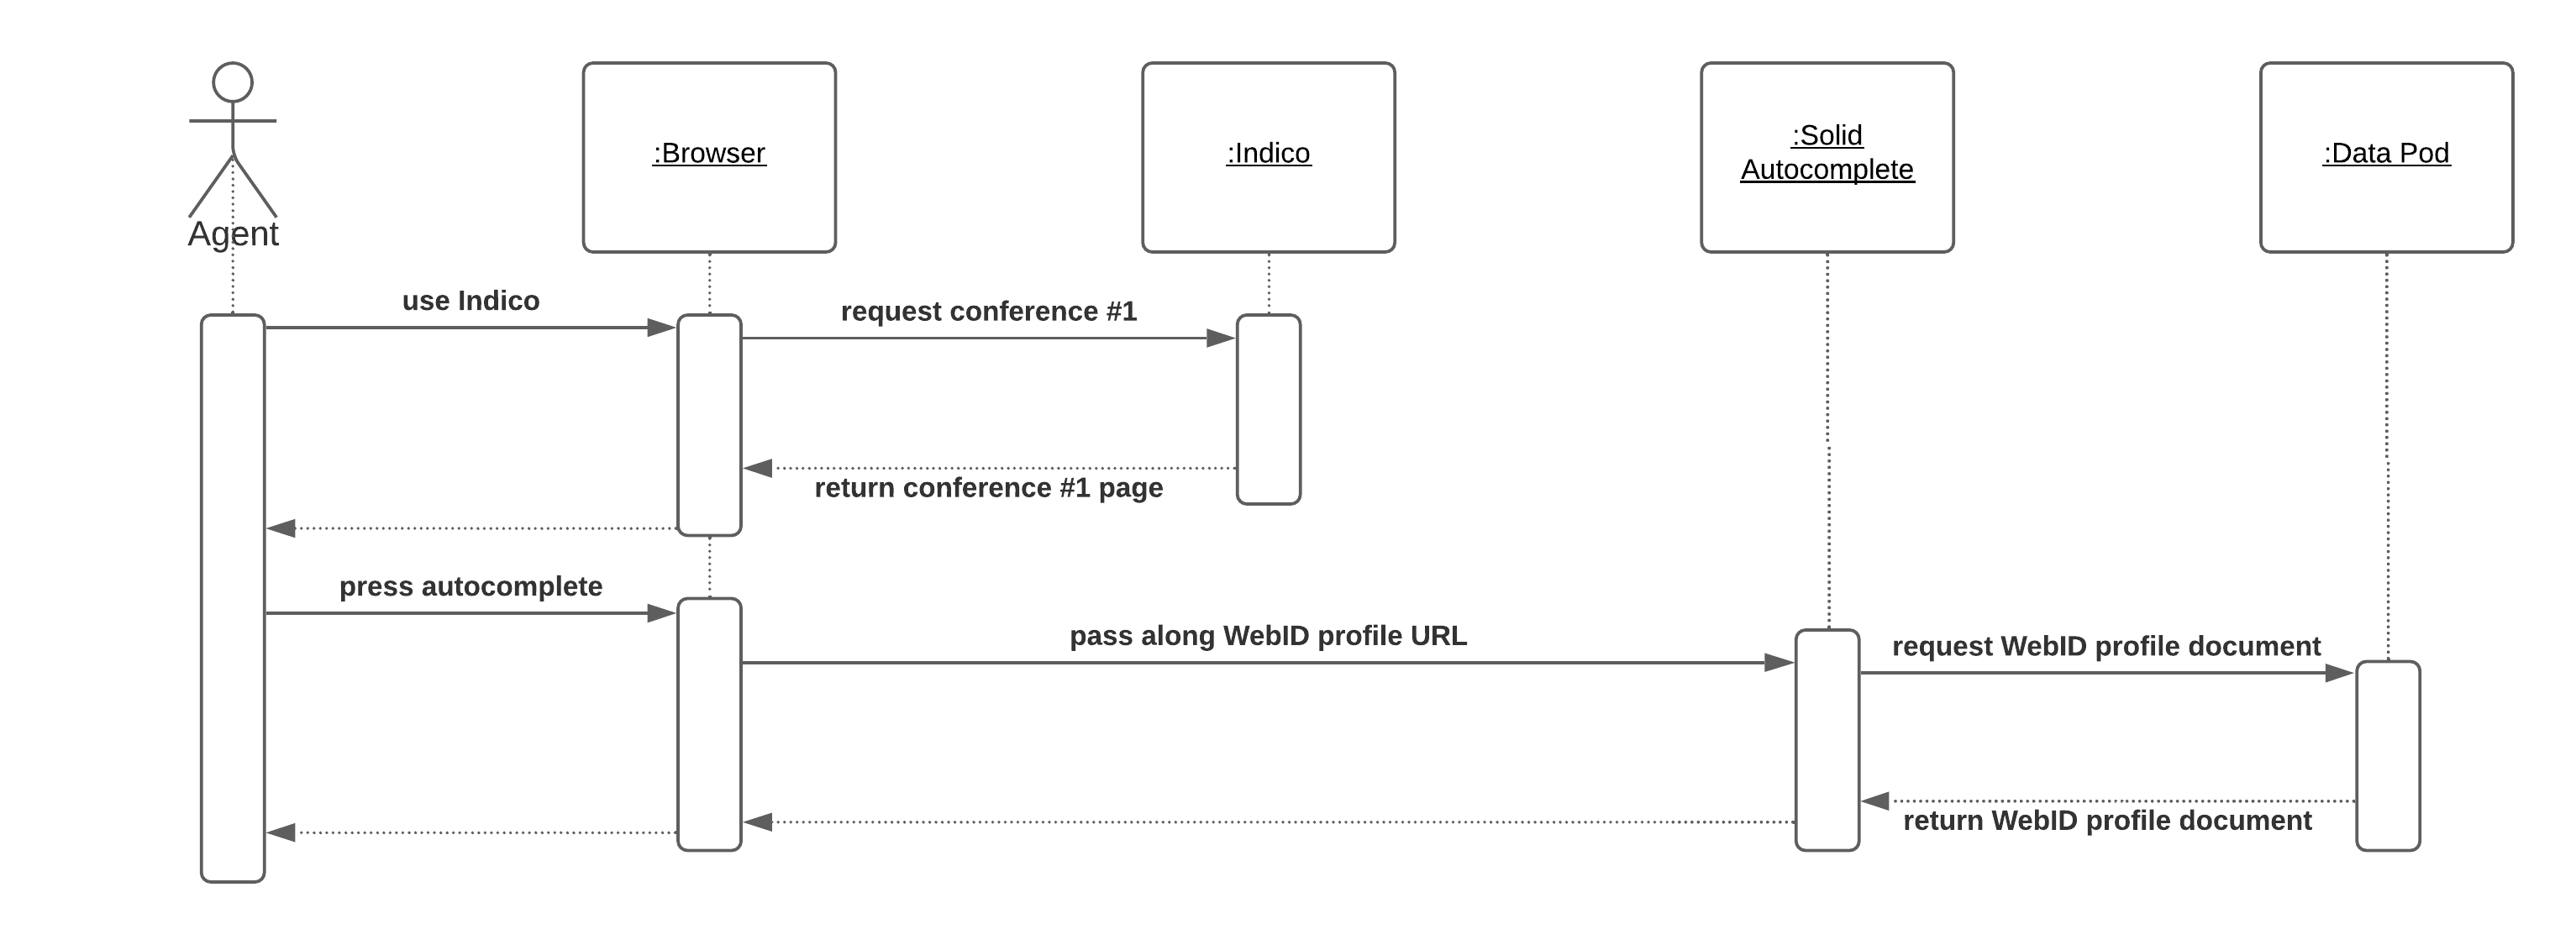
\includegraphics[width=\textwidth]{prototype/graphs/poc-conference_registration-autocomplete-sequence_diagram.png}
    \caption{Sequence diagram showing the sequential process through pulling in data from a data pod.}
    \label{fig:poc-conference_registration-autocomplete-sequence_diagram}
\end{figure}

\vspace{0.5cm}
\paragraph{Stakeholders}\mbox{}\\

TODO:
\vspace{0.5cm}
\paragraph{Drivers}\mbox{}\\

TODO:

\subsubsection{Screen Design}\mbox{}\\

\begin{figure}[ht!]
    \centering
    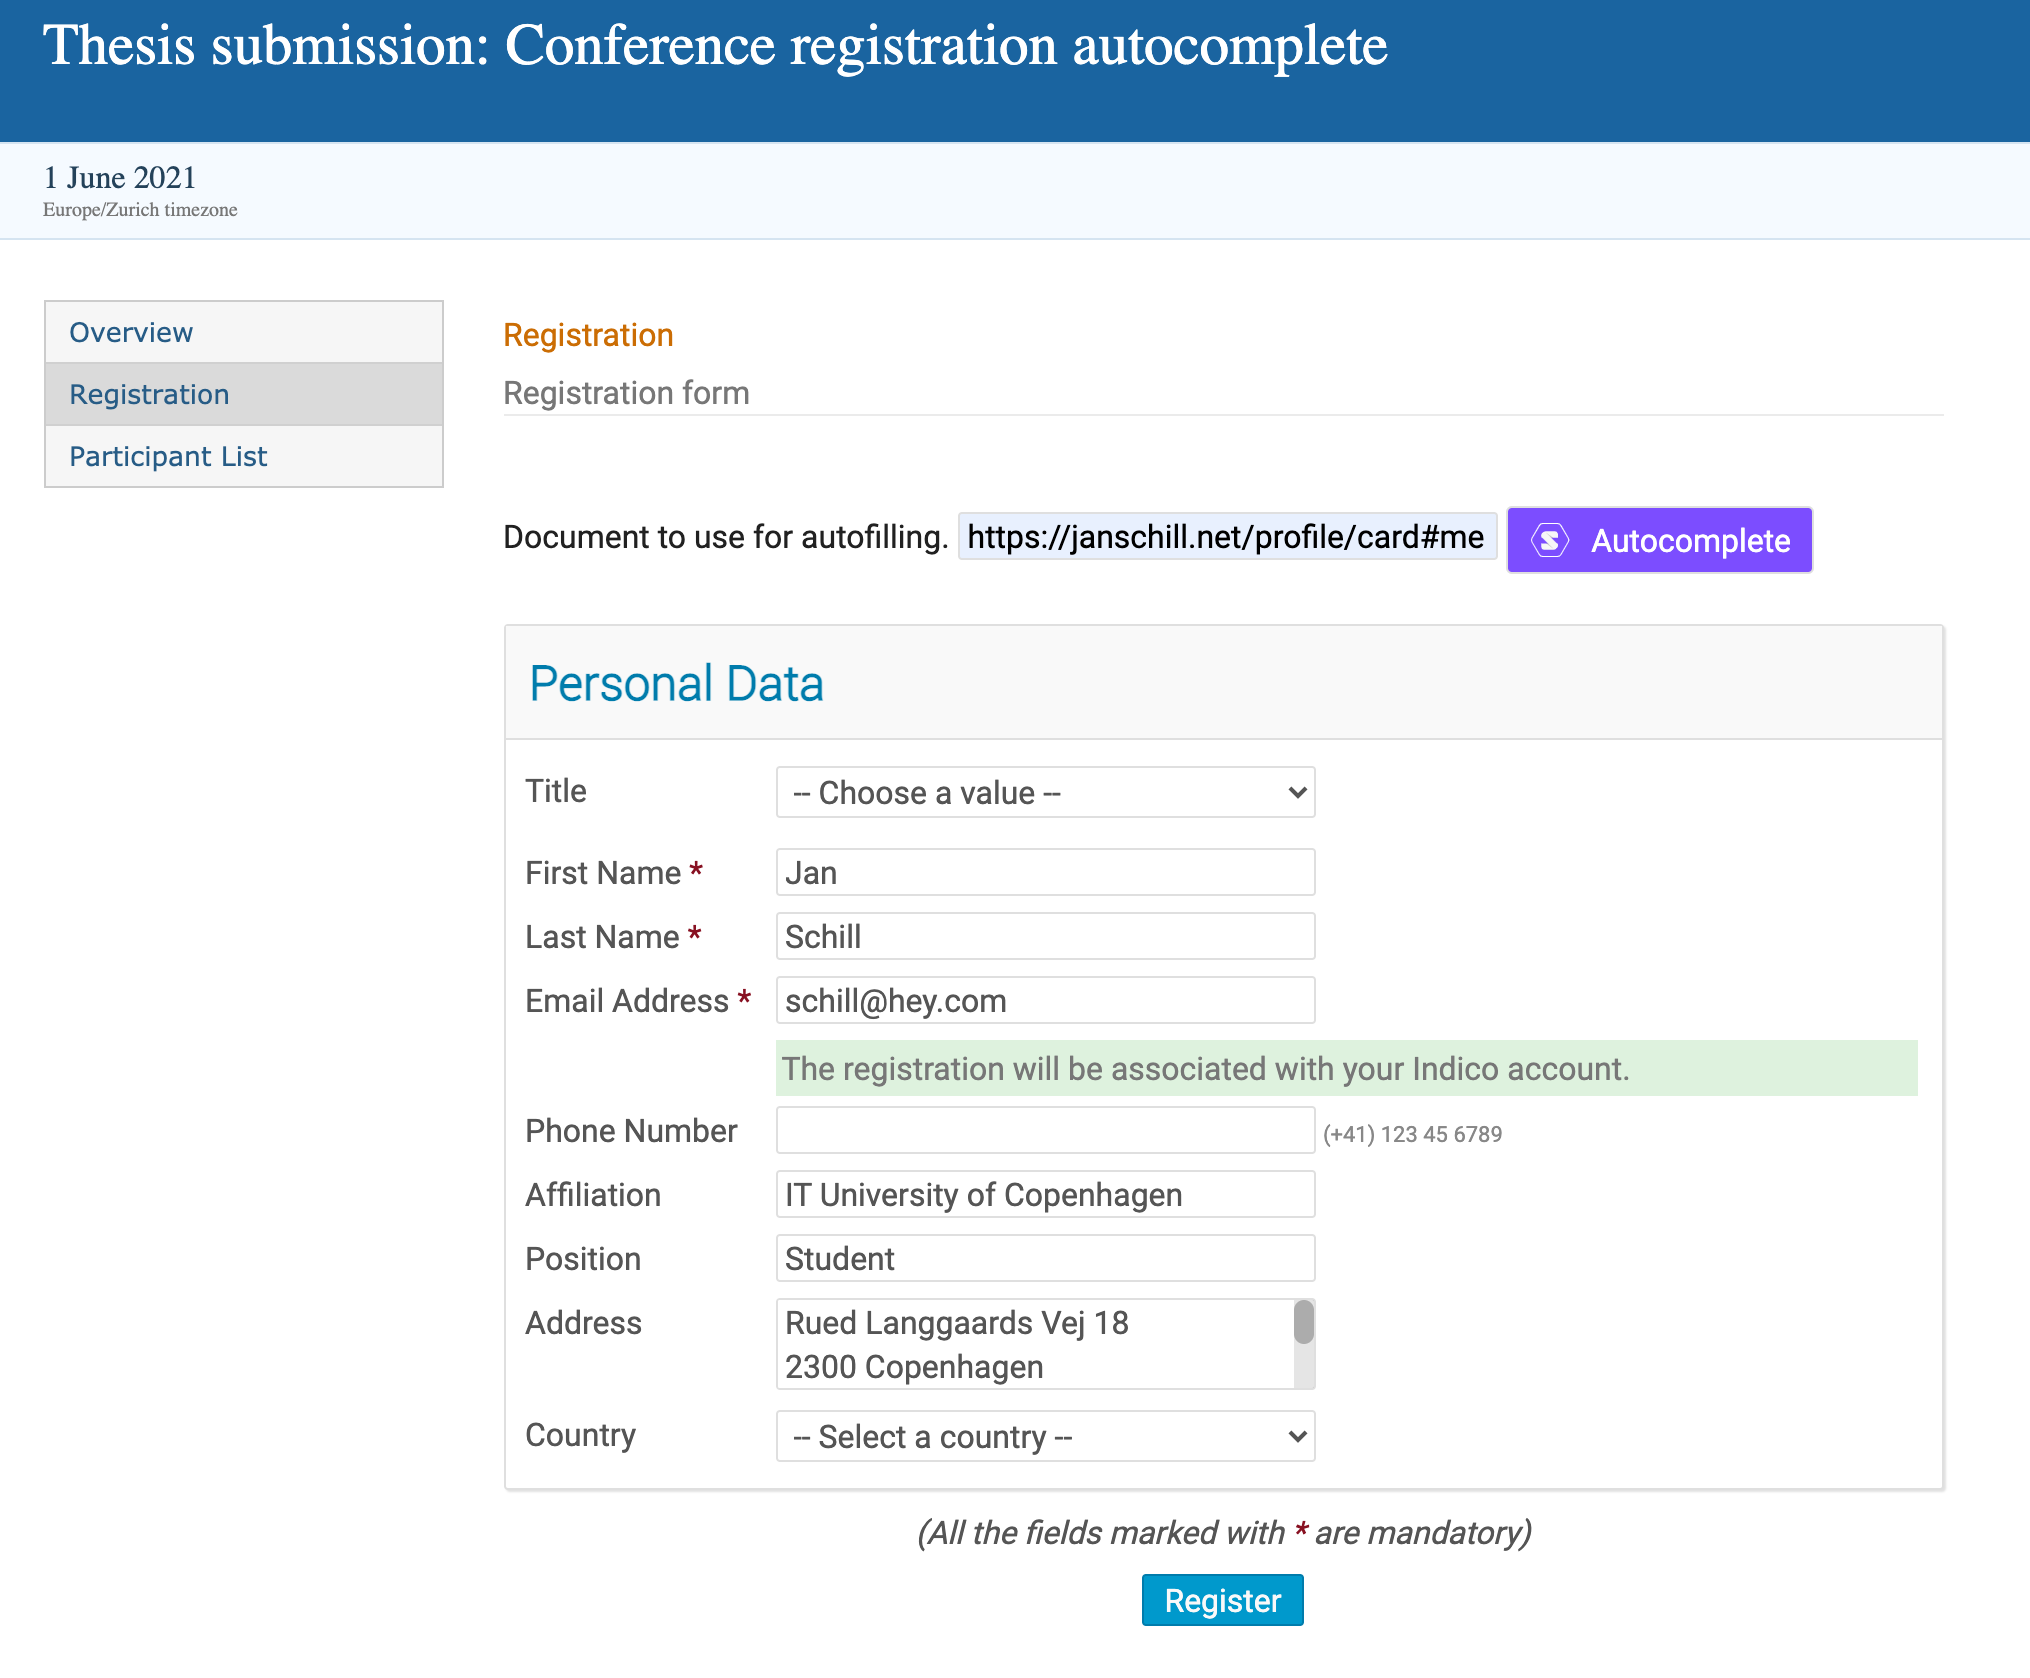
\includegraphics[width=0.75\textwidth]{prototype/graphs/poc-autocomplete-conference-registration.png}
    \caption{User interface showing the comment module: Comments.}
    \label{fig:poc-autocomplete-conference-registration}
\end{figure}

\begin{figure}[ht!]
    \centering
    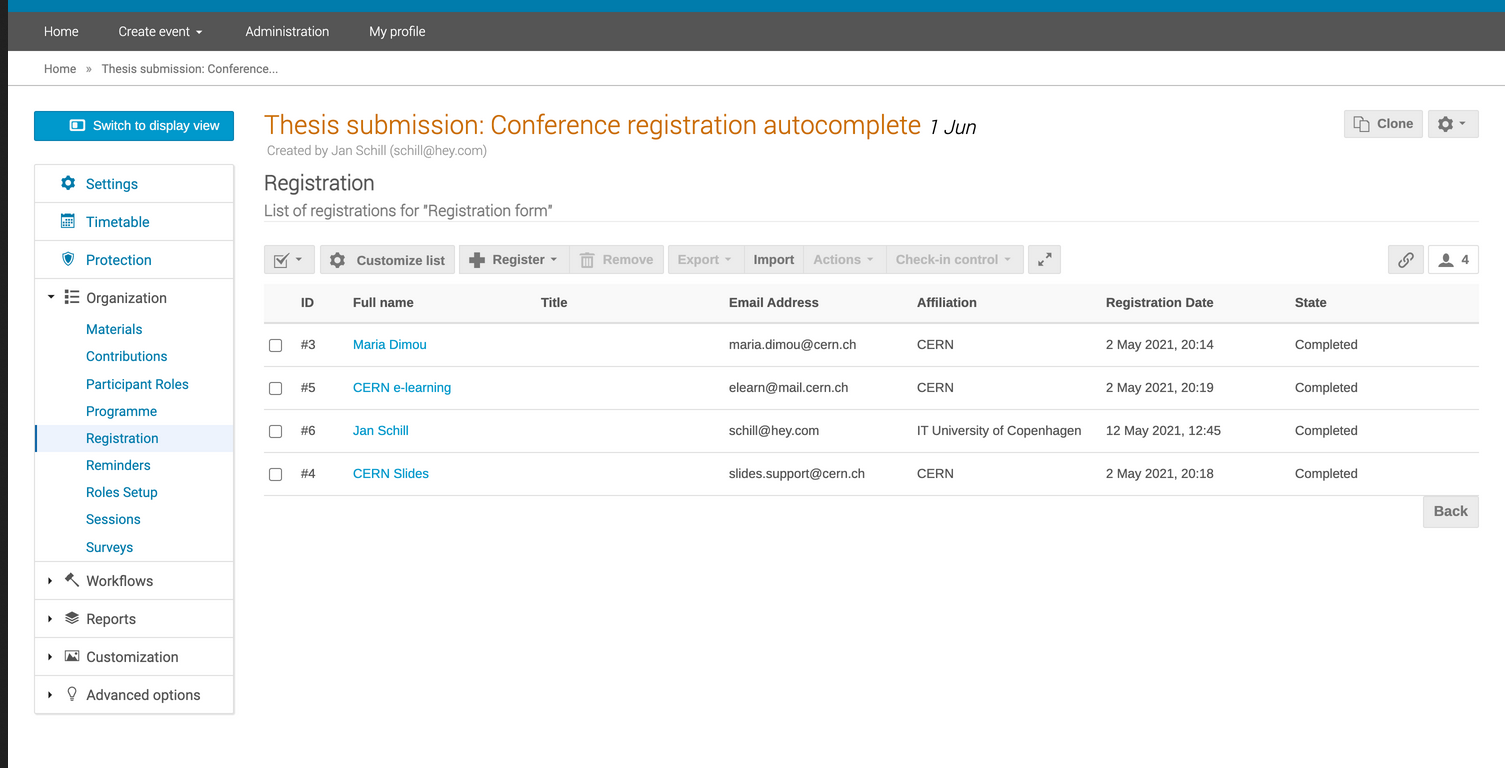
\includegraphics[width=0.75\textwidth]{prototype/poc-solid-autocomplete-conference-registration-attendees.png}
    \caption{User interface showing the comment module: Comments.}
    \label{fig:poc-autocomplete-conference-registration-submitted}
\end{figure}

\subsubsection{Design}\label{poc2:design}\mbox{}\\

The following section will shed light on the design decision made in the process of sketching out the architecture of the module and developing the system. It will introduce the different challenges and how they were overcome. Especially, it will give an explanation of what led to the change of core functionality of the module. In the succeeding section, the choices will be analyzed more explicitly.
\vspace{0.5cm}
\paragraph{Mapping Structured Data To \gls{html} Inputs}\mbox{}\\

A great benefit of using Linked Data is its semantic structure and the interoperability it brings when using in systems supporting it. This means the data are using public vocabularies to be described and thus can be reasoned about by machines and can be move from one system into another one and seamlessly integrated. Indico does not make use of any common \gls{rdf} features and can therefore not extract any of those benefits. Because of this, no simple way of mapping the incoming data from the data pod to the inputs exist, but a few options are feasible.

\begin{enumerate}
    \item Enrich the form with some kind of descriptive indicator
    \item Parse and process existing values of attributes and labels
\end{enumerate}

In the \gls{html} specification an \texttt{autocomplete} attribute exist, which is used by browsers to prefill data from previously used values \cite{html-spec}. The value of the \texttt{autocomplete} key-value pair describes the input and what data is to be expected.

\begin{lstlisting}[language=Other,columns=fullflexible, caption={Autocomplete attribute on input field}, label={lst:autocomplete-input}]
<form method=post action="/">
  <p><label>Full name: <input type=text autocomplete=name></label>
  <p><label>Credit card number: <input type=text inputmode=numeric autocomplete=cc-number></label>
  <p><label>Expiry Date: <input type=month autocomplete=cc-exp></label>
  <p><input type=submit value="Submit">
</form>
\end{lstlisting}

In listing \ref{lst:autocomplete-input} the browser would suggest cached values when the user agent clicks into an input. This is the perfect indicator to \textit{autofill} form inputs. Unfortunately, this attribute is not being utilized in Indico. Another and even better approach would be to annotate the input fields straight up with the vocabulary of for example Schema.org \cite{schema-org}. The mapping of the input fields and the fetched Turtle resource could then happen directly using the \textit{predicates} of both structured formats. To change the AngularJS form and implement new features into Indico were already established not to be viable. Nevertheless, the \texttt{autocomplete} feature shall be kept in mind.

Without being able to extract from the \texttt{autocomplete} attribute within Indico it shall still be implemented and used, as other systems might use the attribute. Other means of extracting some kind of information from the form are the ID and name attributes or even the \texttt{TextNode} of the input label. The ID and name are often equipped with information about the input they are defined on. These values and additionally the value of the label node can be extracted and mapped against a dictionary of key-value pairs to find out what the input is supposed to be filled in with.

\begin{figure}[ht!]
    \centering
    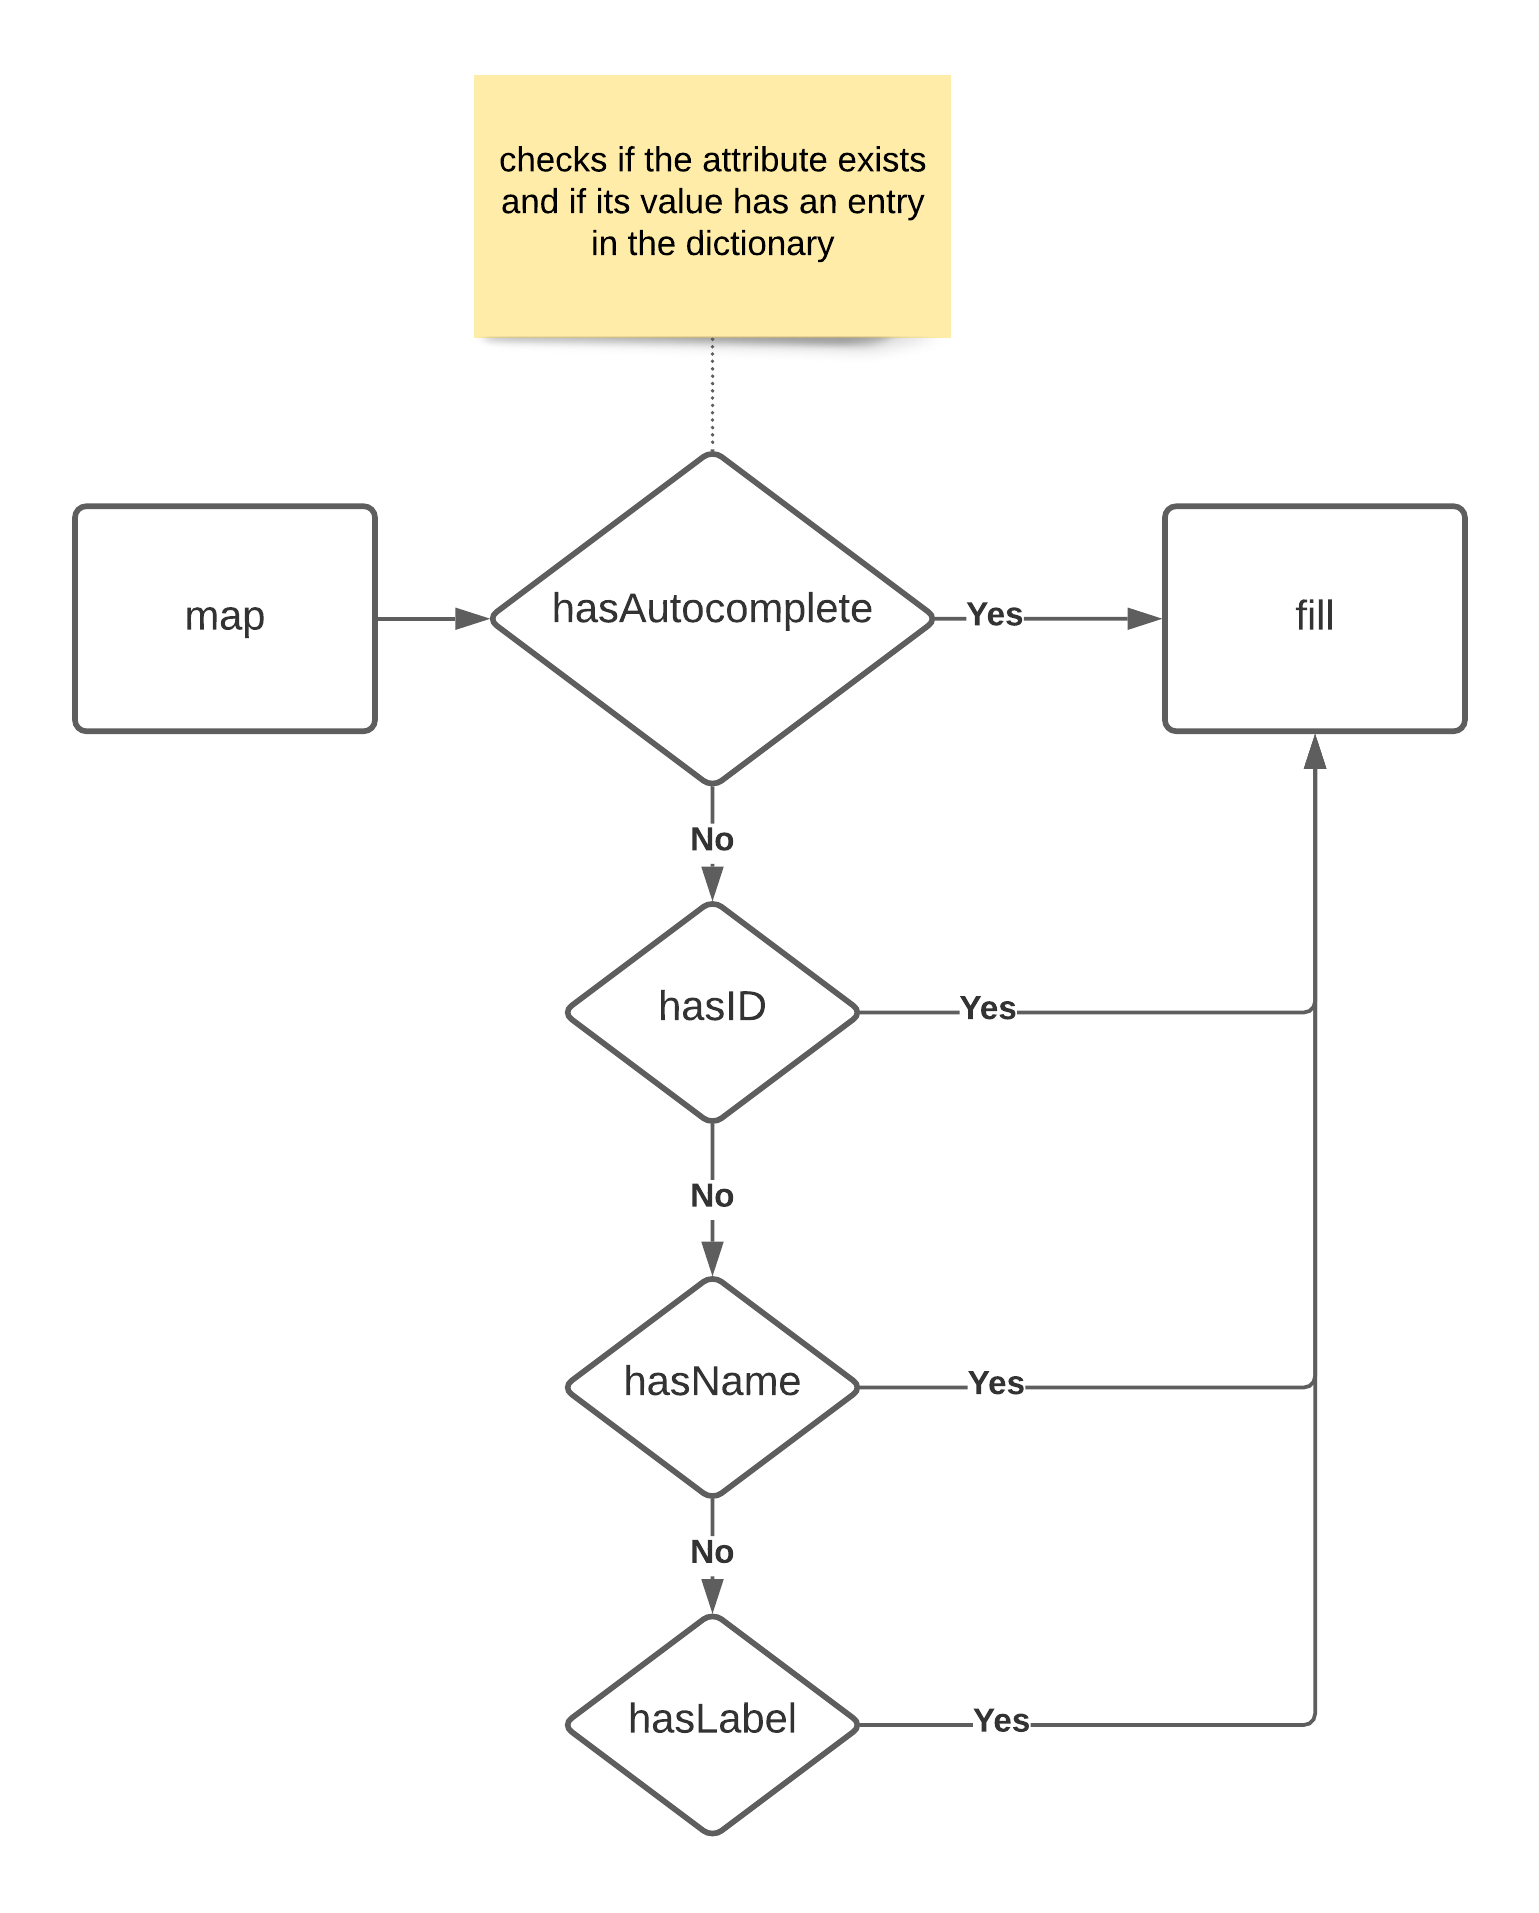
\includegraphics[width=0.5\textwidth]{prototype/graphs/poc-autocomplete-mapping-flow.png}
    \caption{The flow to find a source for dictionary mapping.}
    \label{fig:poc-autocomplete-mapping-flow}
\end{figure}

A possible mapping of address information could look like as in listing \ref{lst:autocomplete-mapping}. The implementation shows a \gls{js} implementation where the key in the \texttt{address} object are the possibly extracted values from the different techniques described above and the value is in this example the vCARD \cite{vcard-spec} equivalent. vCARD is being used by the \gls{nss} to describe the information in the WebID profile document.

\begin{lstlisting}[language=Other,columns=fullflexible, caption={Dictionary to map extracted values with predicates from Turtle resource}, label={lst:autocomplete-mapping}]
const address = {
  address: 'full_address',
  country: VCARD.country_name.value,
  countryName: VCARD.country_name.value,
  region: VCARD.region.value,
  locality: VCARD.locality.value,
  city: VCARD.locality.value,
  streetAddress: VCARD.street_address.value,
  street: VCARD.street_address.value,
  postalCode: VCARD.postal_code.value
}
\end{lstlisting}

Listing \ref{lst:webid-address} shows part of the WebID profile document where the address of an agent is described.

\begin{lstlisting}[language=Other,columns=fullflexible, caption={Extraction from WebID profile document showing address.}, label={lst:webid-address}]
@prefix : <#>.
@prefix n: <http://www.w3.org/2006/vcard/ns#>.
# ...
:id1614172452178
  n:country-name "Denmark";
  n:locality "Copenhagen";
  n:postal-code "2300";
  n:region "Zealand";
  n:street-address "Rued Langgaards Vej 18". 
# ...
:me n:hasAddress :id1614172452178;
# ...
\end{lstlisting}

\vspace{0.5cm}
\subsubsection{Integration With Indico}\mbox{}\\

A few challenges arose when integrating the module with Indico. A critical issue was when it was found out that the form is not rendered on the server and send as \gls{html} in the response body as expected. Another challenge was when programmatically filling in the input fields of the inputs the frontend form validation would not detect a change in the input values and thus would think no input value is given.

\vspace{0.5cm}
\paragraph{Bind to Dynamically Created Form}\mbox{}\\

Indico builds the registration form dynamically using a frontend library called AngularJS \cite{angularjs}. This introduces a challenge of interacting with the form using \gls{js}. Frontend libraries that either create new or modify existing \gls{dom} nodes need to wait until the complete \gls{dom} tree is loaded, as they bind to one \gls{dom} node from the initially served \gls{html} document and then do their operations on this node. Meaning, AngularJS waits until the whole \gls{html} document is parsed and rendered in the browser and then starts creating its form from scratch, which is then being rendered by the browser. The problem with this is in order to operate on the form, which is necessary for the module to be able to read the form inputs and labels and also to set their values, the \gls{js} code from this prototype needs to know when the form was successfully rendered. Three options are possible to achieve this.

\begin{enumerate}
    \item Implement the autocomplete functionality in the existing AngularJS form code
    \item Dispatch an event to notify the autocomplete module the form has been rendered
    \item Use the \texttt{MutationObserver} to detect the form creation
\end{enumerate}

Solutions 1 and 2 both involve the need to work with the AngularJS form, which is written in a legacy version and was recommended by an Indico developer to -- if possible -- be avoided. Indico developers also plan on removing AngularJS altogether and replace it with a more popular frontend framework. Therefore, option 3 was chosen even though the usage of a \texttt{MutationObserver} instance might add performance degradation to the page load \cite{dom-spec}. The performance shall not be analyzed more carefully as it is not of relevance to prove the realization of the prototype.

The \texttt{MutationObserver} is initialized as soon as the \gls{dom} is rendered, it then takes a node as a target to observe and will register all modifications on this node: the creation of children nodes in it, updates to the node itself or any other modifications. To reduce computation the Indico code can be analyzed to find a suitable \gls{dom} element to have as a target node. This node needs to exist when the \gls{dom} is loaded and needs to contain the final form node. When looking at the final rendered document containing the AngularJS form one notices that the form has an ID, which can be used to observe its creation.
 
\begin{lstlisting}[language=Other,columns=fullflexible, caption={Observe function in Indico}, label={lst:indico-observe}]
function observeFormCreation() {
  // ID of the AngularJS form, its creation needs to be observed
  const formId = 'registrationForm';
  // Candidate to limit observing scope
  const $conferencePage = document.querySelector('.conference-page');
  const targetNode = $conferencePage;
  // Only observe nodes, not attributes
  const config = {attributes: false, childList: true, subtree: true};

  const callback = (mutationsList, observer) => {
    // Contains all mutations in the targetNode
    for (const mutation of mutationsList) {
      // Node has beed added or removed
      if (mutation.type === 'childList') {
        // Look at all added nodes
        for (const node of mutation.addedNodes) {
          // Look for the AngularJS form
          if (node.id === formId) {
            // Once found, stop observing
            observer.disconnect();
            // Initialize the autocomplete library
            const solidAutocomplete = new SolidAutocomplete({form: node});
            solidAutocomplete.createAutocompleteDomControls(node);
          }
        }
      }
    }
  };
  // Start observing
  const observer = new MutationObserver(callback);
  observer.observe(targetNode, config)
}
\end{lstlisting}

\vspace{0.5cm}
\paragraph{Detect Input Change for Frontend Validation}\mbox{}\\

Indico deploys a frontend validation to make sure it receives proper values for the form's inputs. A basic validation is the check for a presence of values in required inputs. This way Indico can render a hint on the input fields with invalid values, such as if no input was given in a required email address field. It turns out Indico has \texttt{\gls{dom} Event Listeners} which detect if an input field is clicked in and if it is receiving inputs through a user typing in it. This validation implementation does not detect when changing the value of the \texttt{value} attribute of an input node, thus complaining when setting the values through \gls{js}.

\begin{lstlisting}[language=Other,columns=fullflexible, caption={Changing the value of an input node.}, label={lst:input-change}]
const formInputField = document.querySelector('.exampleFormInput')
formInputField.value = 'New value'
\end{lstlisting}

The example code in listing \ref{lst:input-change} would not be detected by Indico and would upon submission render a missing value hint.

Two ways of fixing the problem are conceivable.

\begin{enumerate}
    \item Change Indico frontend validation to detect value change
    \item Dispatch event when setting values in the autocomplete module
\end{enumerate}

Changing the Indico frontend validation might turn out to be more time-consuming than anticipated and is therefore not viable, also it is unknown if a change is wanted by the Indico development team in the first place. The idea for a working implementation is to validate on submission of the form instead of validation when a change on the input is detected. As mentioned before the problem with the used \texttt{oninput} event is it does not detect when the value is set programmatically. If the validation is only happening when the values are tried to be sent to the server by submission the input values can be parsed and the correct value is detected -- no matter how it was set. 

The other and also picked solution is to trigger the \texttt{oninput} event that is being listened on by the Indico validation. The event dispatch needs to happen as soon the values are set within the module and because this happens in the module and the module is a self-contained module without any knowledge of Indico, the module should not be directly changed, but rather allow a callback function to be passed to it and then execute when appropriate.

\begin{lstlisting}[language=Other,columns=fullflexible, caption={Dispatching the \texttt{oninput} event within a callback.}, label={lst:oninput-callback}]
function triggerInputEvent(inputs) {
  for (let i = 0; i < inputs.length; i++) {
    const element = inputs[i];
    [element, element.parentNode].forEach(node => {
      if ('createEvent' in document) {
        const evt = document.createEvent('HTMLEvents');
        evt.initEvent('input', false, true);
        node.dispatchEvent(evt);
      } else {
        node.fireEvent('oninput');
      }
    });
  }
}
\end{lstlisting}

\subsubsection{Evaluation}\mbox{}\\

TODO:
\vspace{0.5cm}
\paragraph{Metrics}\mbox{}\\

TODO:
\vspace{0.5cm}
\paragraph{Levels}\mbox{}\\

The same levels 1 to 5 as in the first evaluation \ref{section:poc1-evaluation} will be used to rate the architecture of this system.
\vspace{0.5cm}
\paragraph{Components}\mbox{}\\

TODO:
\vspace{0.5cm}
\subsubsection{Analysis}\label{poc2:analysis}\mbox{}\\

The analysis of the second \gls{poc} will focus on the original design idea and what led to a change of mind. It will do so by looking at the relevant modules in Indico that caused the direction for the \gls{poc} to alter. It will also be analyzed, what role Solid's design played in the abandonment of the idea on storing the registration data in data pods and effectively giving up usage control.



* Gave up usage control
  * Why it didn't work, and **what is necessary to make it work**
    * usage control
    * question the choice of Indico usage control
    * versioning of tag of personal data
* high-level constraints
* implementation
  * indico limits this
* if indico in this way or more generally

\vspace{0.5cm}
\paragraph{Iterations}\mbox{}\\
TODO:
1st iteration, save data in pod
2nd iteration, only pull data from pod

TODO: Include these somehow:

\begin{figure}
    \centering
    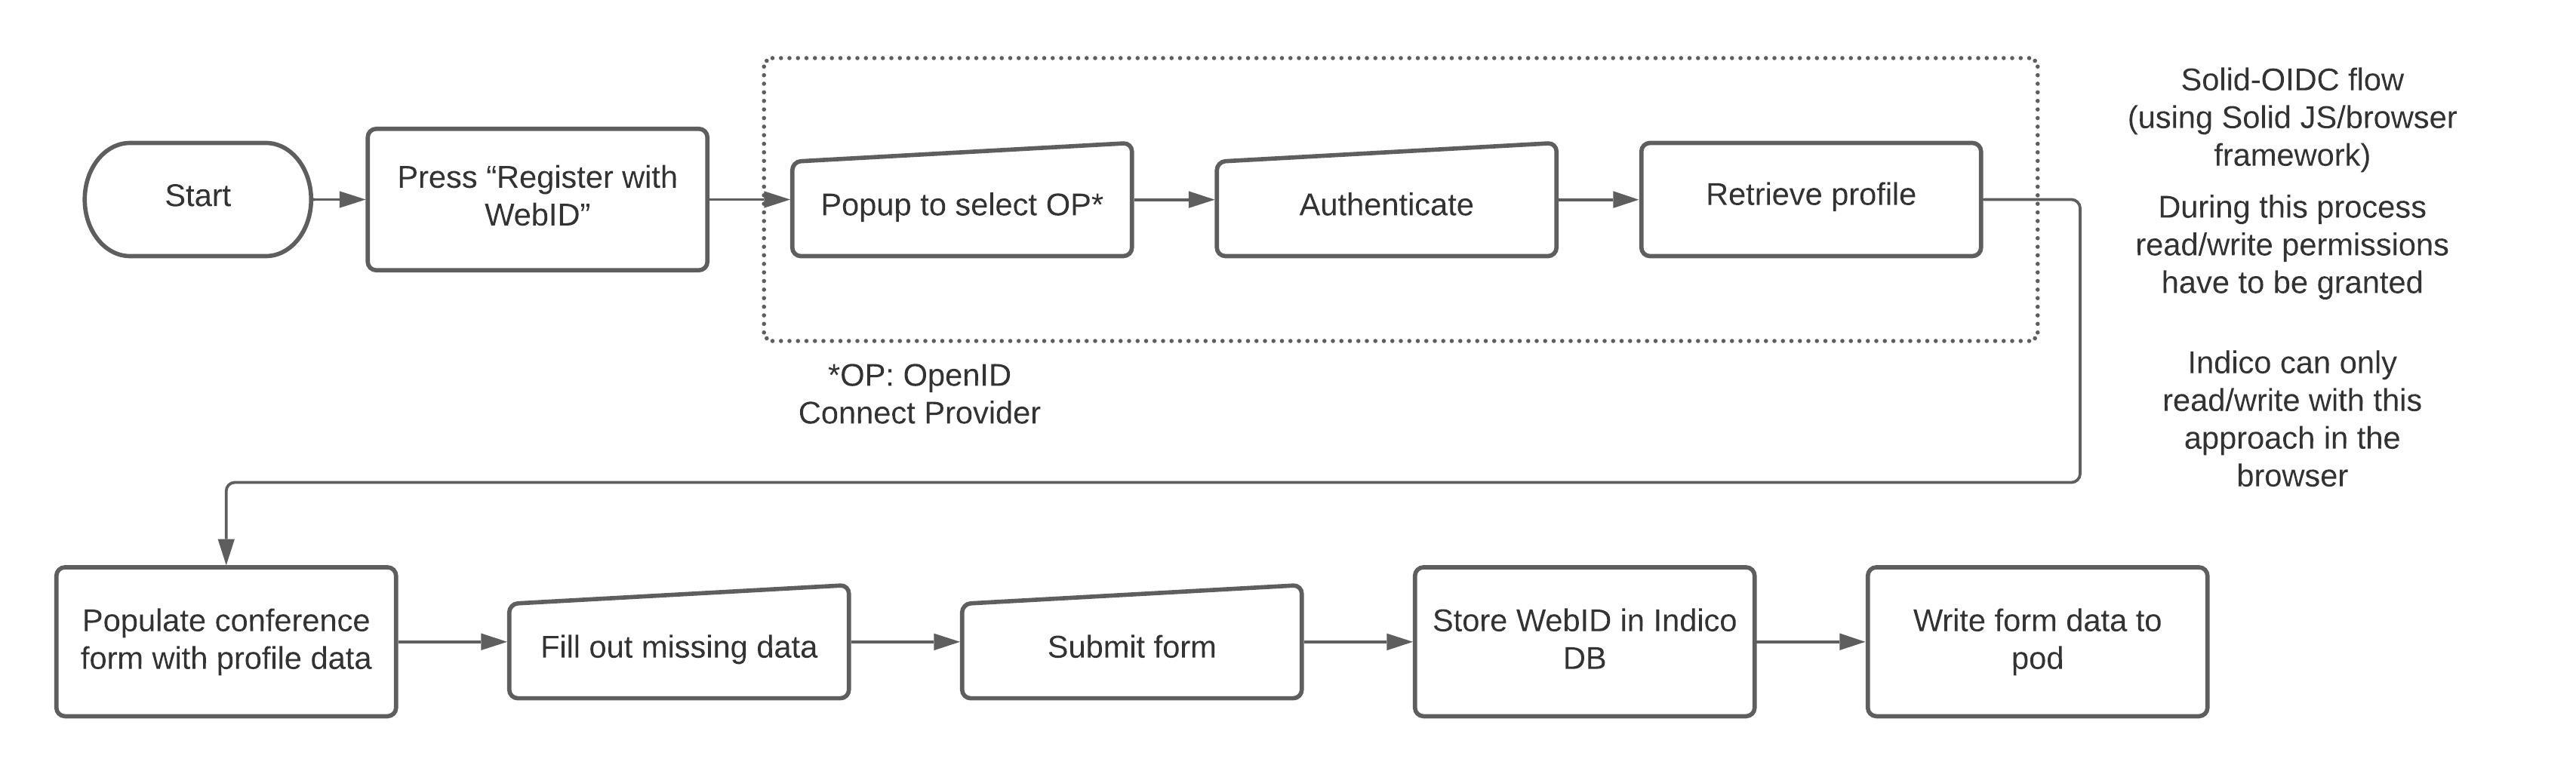
\includegraphics[width=1\textwidth]{prototype/graphs/poc-conference_registration_flow-client_side-sideways.jpeg}
    \caption{TODO:}
    \label{fig:poc-conference_registration_flow-client_side-sideways}
\end{figure}

\begin{figure}
    \centering
    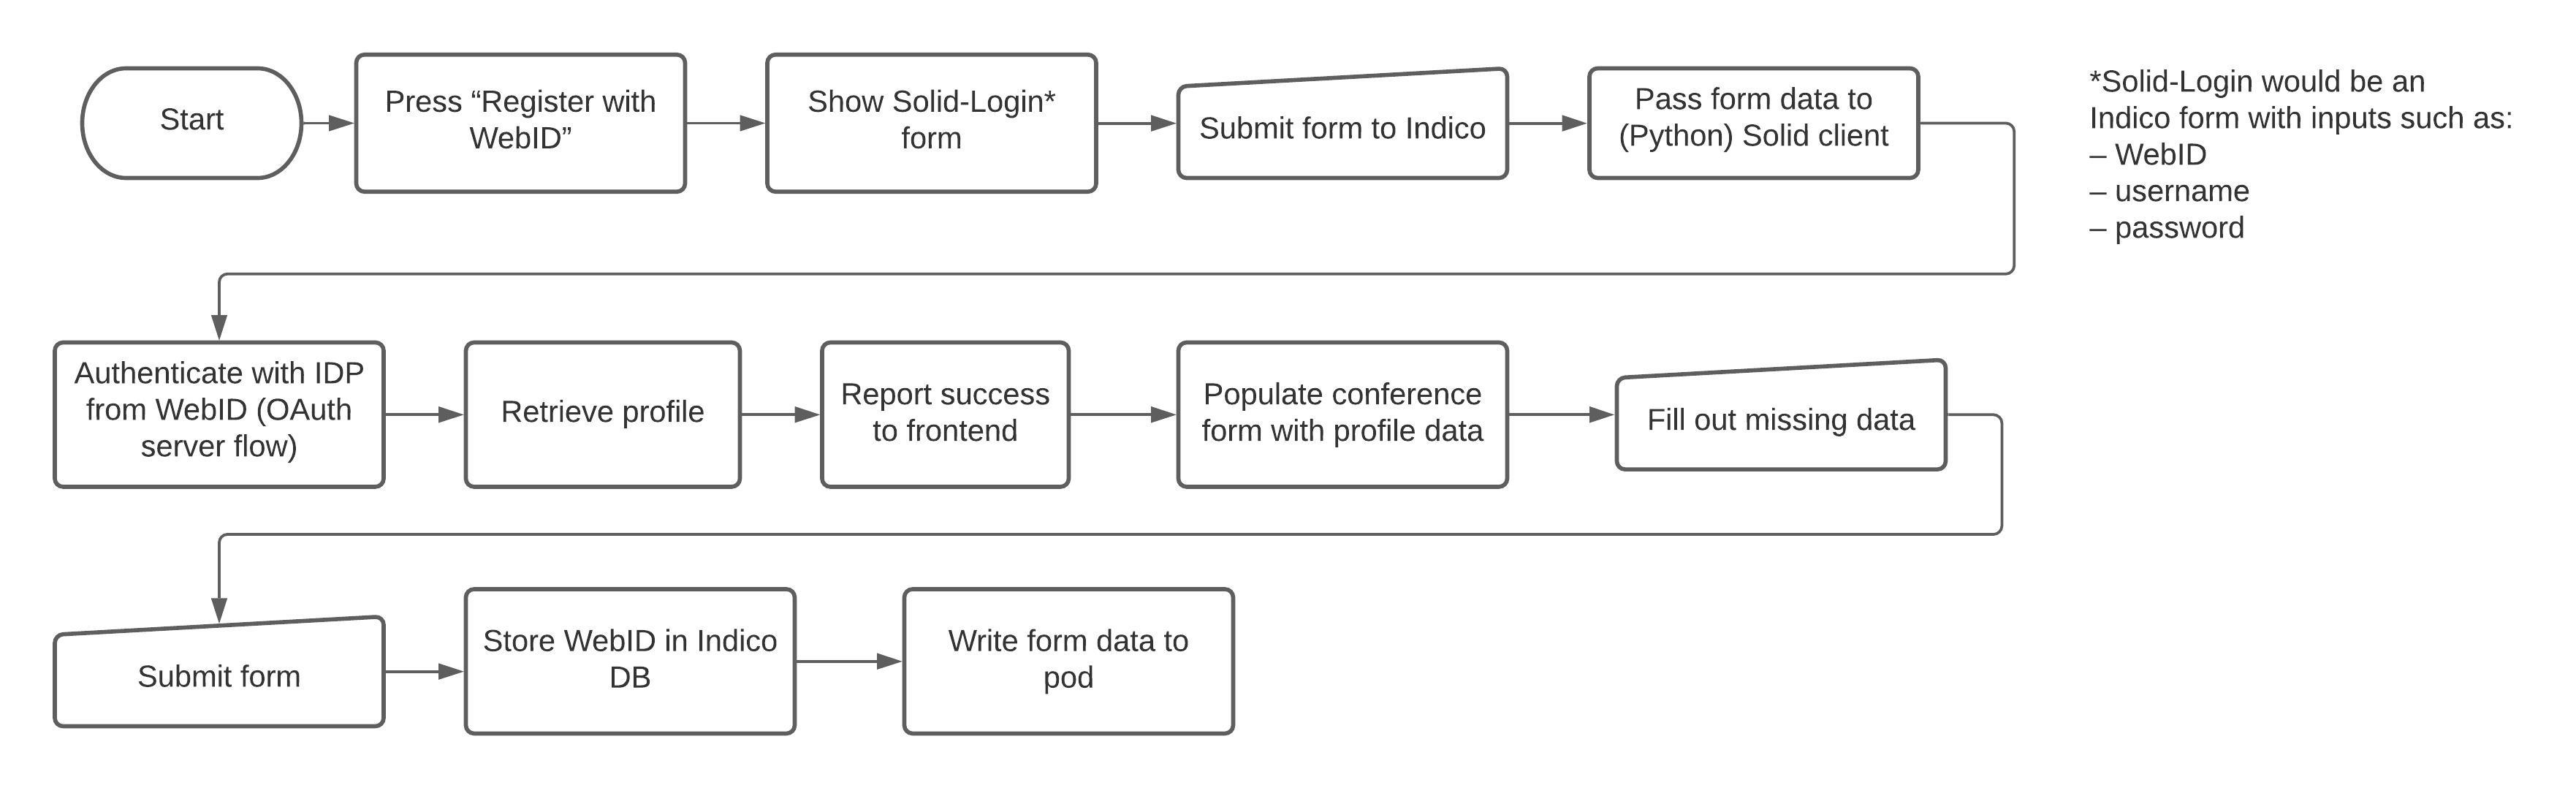
\includegraphics[width=1\textwidth]{prototype/graphs/poc-conference_registration_flow-server_side-sideways.jpeg}
    \caption{TODO:}
    \label{fig:poc-conference_registration_flow-server_side-sideways}
\end{figure}

\begin{figure}
    \centering
    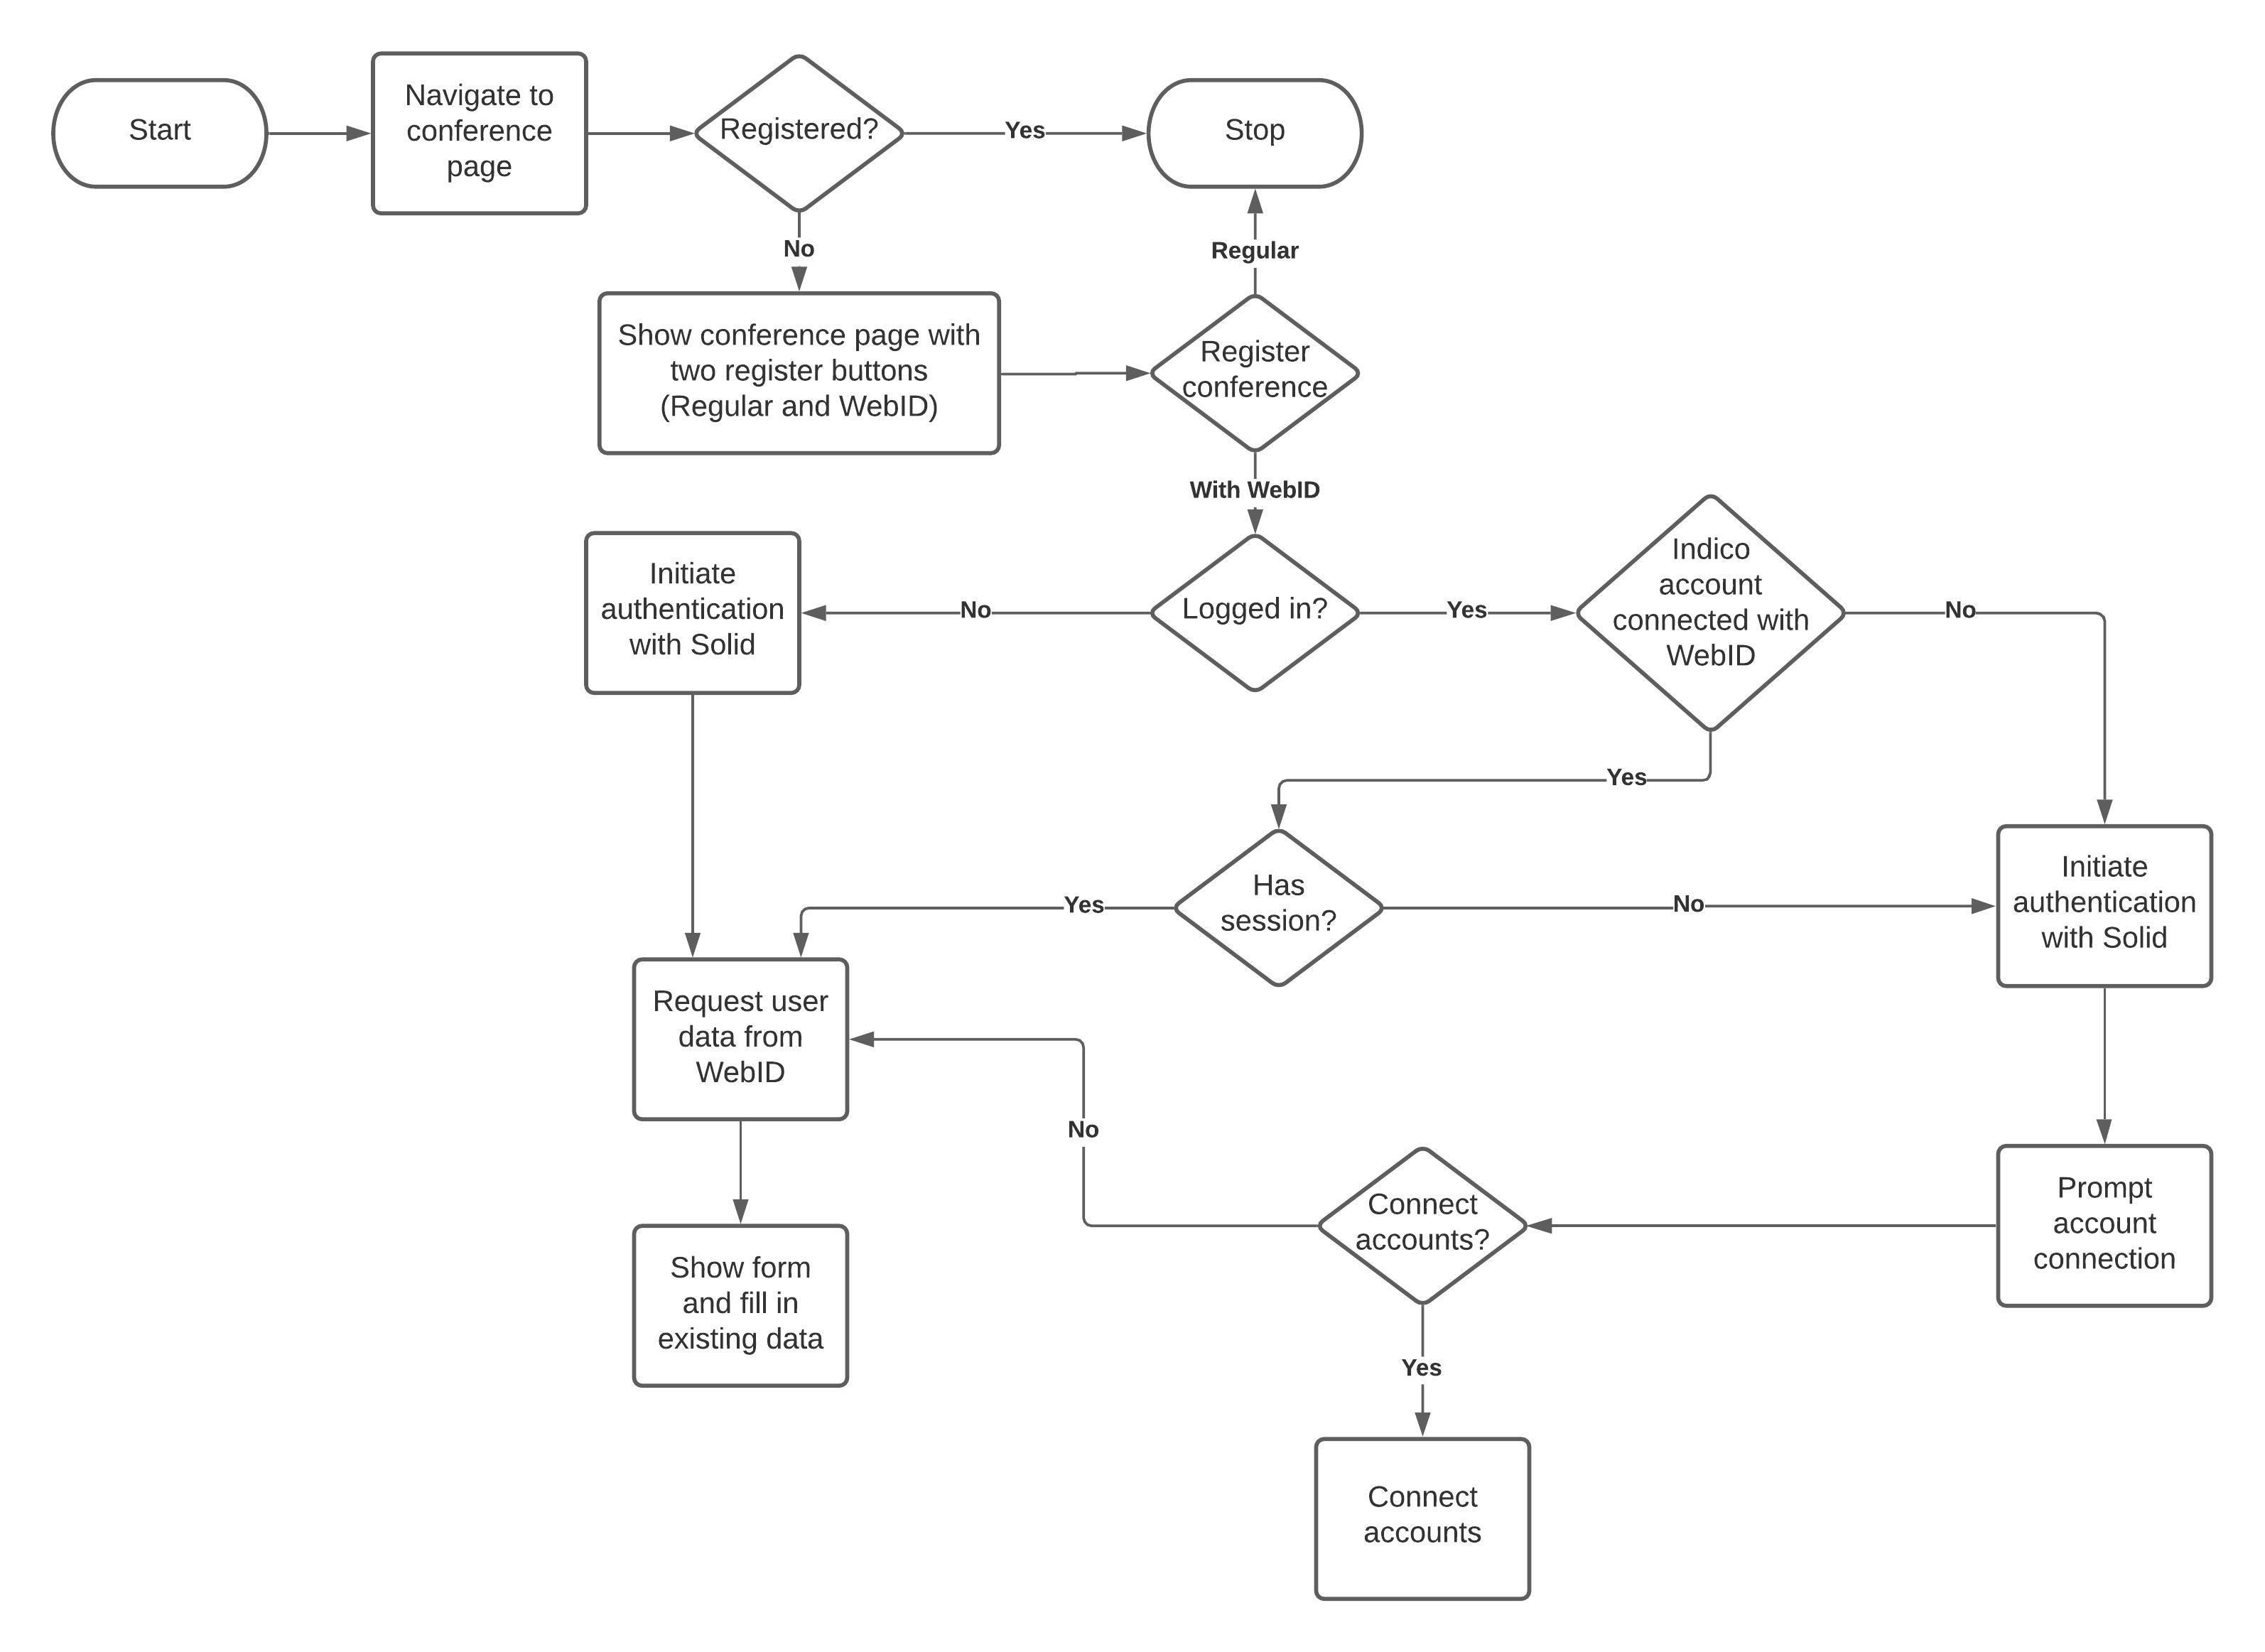
\includegraphics[width=1\textwidth]{prototype/graphs/poc-conference_registration_flow-sideways.jpeg}
    \caption{TODO:}
    \label{fig:poc-conference_registration_flow-sideways}
\end{figure}
\vspace{0.5cm}
\paragraph{Modification of Resource From Data Pod}\mbox{}\\

TODO:
\vspace{0.5cm}
\paragraph{Payment on Input Fields}\mbox{}\\

TODO:
\vspace{0.5cm}
\paragraph{Performance of Large Conference}\mbox{}\\

TODO:
\vspace{0.5cm}
\paragraph{Availability of Crucial User Data}\mbox{}\\

TODO:


* performance?
* Management part of Indico
  * Forward data between people
  * **Also serve data to people (admin of registration)**
* Comments are more clear tied to comment?

* the flow of Solid (ref Tim from White Area) notifying for future conference
* Indico does not have any RDF semantically structured data